\thispagestyle{empty}

\noindent%
\begin{tabularx}{\textwidth}{@{}lXr@{}}%
    & & \large{На правах рукописи}\\
    \IfFileExists{}{
\includegraphics[height=2.5cm]{logo}}{\rule[0pt]{0pt}{2.5cm}}  & &
    \ifnumequal{\value{showperssign}}{0}{%
        \rule[0pt]{0pt}{1.5cm}
    }{
        \includegraphics[height=1.5cm]{}
    }\\
\end{tabularx}

\vspace{0pt plus1fill} %число перед fill = кратность относительно некоторого расстояния fill, кусками которого заполнены пустые места
\begin{center}
\textbf {\large \thesisAuthor}
\end{center}

\vspace{0pt plus3fill} %число перед fill = кратность относительно некоторого расстояния fill, кусками которого заполнены пустые места
\begin{center}
\textbf {\Large %\MakeUppercase
\thesisTitle}

\vspace{0pt plus3fill} %число перед fill = кратность относительно некоторого расстояния fill, кусками которого заполнены пустые места
{\large Специальность \thesisSpecialtyNumber\ "---\par <<\thesisSpecialtyTitle>>}

\vspace{0pt plus1.5fill} %число перед fill = кратность относительно некоторого расстояния fill, кусками которого заполнены пустые места
\Large{Автореферат}\par
\large{диссертации на соискание учёной степени\par \thesisDegree}
\end{center}

\vspace{0pt plus4fill} %число перед fill = кратность относительно некоторого расстояния fill, кусками которого заполнены пустые места
{\centering\thesisCity~--- \thesisYear\par}

\newpage
% оборотная сторона обложки
\thispagestyle{empty}
\noindent Работа выполнена в {\thesisInOrganization}.


\noindent%

\textbf{Научный консультант:}

\textit{Лаврентьев Михаил Михайлович}

доктор физико-математических наук, профессор, федеральное государственное автономное образовательное учреждение высшего образования «Новосибирский национальный исследовательский государственный университет», декан факультета информационных технологий.

\vspace{0.004\paperheight plus1fill}
\noindent%

\textbf{Официальные оппоненты:}

\textit{Воеводин Владимир Валентинович}

доктор физико-математических наук, член-корреспондент РАН,
федеральное государственное бюджетное образовательное учреждение высшего образования «Московский государственный университет имени
М.В. Ломоносова», заместитель директора научно-исследовательского вычислительного центра

\vspace{0.004\paperheight plus1fill}
\textit{Калайда Владимир Тимофеевич}

доктор технических наук, профессор, федеральное государственное автономное
образовательное учреждение высшего образования «Национальный
исследовательский Томский государственный университет»,
профессор кафедры оптико-электронных систем и дистанционного
зондирования.

\vspace{0.004\paperheight plus1fill}
\textit{Рояк Михаил Эммануилович}

доктор технических наук, профессор, федеральное государственное бюджетное образовательное учреждение высшего образования Новосибирский государственный технический университет, профессор кафедры прикладной математики.

\vspace{0.004\paperheight plus1fill}
\textbf{Ведущая организация} - Федеральное государственное бюджетное учреждение науки Институт гидродинамики им. М.А. Лаврентьева Сибирского отделения Российской академии наук.


\vspace{0.004\paperheight plus1fill}

\noindent Защита состоится \defenseDate~на~заседании диссертационного совета \defenseCouncilNumber~ \defenseCouncilTitle~по адресу: \defenseCouncilAddress.

\vspace{0.004\paperheight plus1fill}
\noindent С диссертацией можно ознакомиться в библиотеке \synopsisLibrary.

\vspace{0.004\paperheight}


Автореферат разослан «   »\_\_\_\_\_\_ 2019 г.


\vspace{0.008\paperheight plus1fill}
\noindent%
\begin{tabularx}{\textwidth}{@{}%
>{\raggedright\arraybackslash}b{18em}@{}
>{\centering\arraybackslash}X
r
@{}}
    Ученый секретарь\par
    диссертационного совета
    \defenseCouncilNumber,\par
    \defenseSecretaryRegalia
    &
    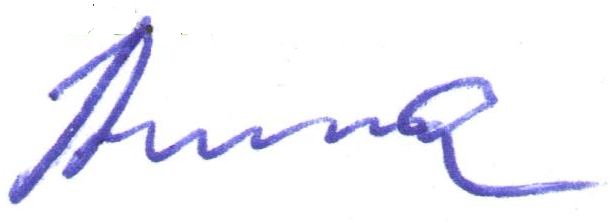
\includegraphics[height=1.0cm]{secretary-signature.png}
    &
    \defenseSecretaryFio
\end{tabularx}
